\section{Mô hình Sinh video từ Văn bản (Text-to-Video)}
\label{sec:text_to_video}

\subsection{Tổng quan: Từ Khoảnh khắc đến Câu chuyện}
\label{subsec:t2v_overview}
Nếu các mô hình Text-to-Image như Stable Diffusion đã trao cho chúng ta khả năng biến ngôn từ thành những khoảnh khắc tĩnh, thì các mô hình \textbf{Tạo video từ Văn bản (Text-to-Video - T2V)} là bước nhảy vọt tiếp theo, thổi hồn vào những khoảnh khắc đó bằng \textbf{chuyển động, thời gian và cốt truyện}. Đây là một trong những lĩnh vực nghiên cứu và ứng dụng bùng nổ nhất trong giai đoạn 2023-2025, hứa hẹn sẽ định hình lại ngành công nghiệp sáng tạo nội dung, điện ảnh, và marketing.

Tuy nhiên, việc chuyển từ ảnh sang video không chỉ đơn giản là tạo ra một chuỗi các ảnh riêng lẻ. Thách thức lớn nhất và cốt lõi nhất của T2V là \textbf{tính nhất quán theo thời gian (temporal consistency)}. Làm thế nào để đảm bảo một nhân vật giữ nguyên ngoại hình qua các khung hình? Làm thế nào để các vật thể di chuyển một cách hợp lý về mặt vật lý và tương tác với nhau một cách có ý nghĩa? Làm thế nào để duy trì một bối cảnh và phong cách nghệ thuật xuyên suốt cả đoạn video?

Giải quyết những thách thức này đòi hỏi một sự kết hợp tinh vi giữa các kiến trúc sinh mạnh mẽ (thường là Diffusion Models hoặc Transformer) và các cơ chế mô hình hóa động học và thời gian phức tạp.

\subsection{Các Nguyên lý Kiến trúc chung}
\label{subsec:t2v_architectural_principles}
Hầu hết các mô hình T2V hiện đại đều được xây dựng dựa trên một kiến trúc nền tảng, kế thừa từ thành công của các mô hình T2I như Latent Diffusion Models (LDM).
\begin{mdframed}[style=infobox]
	\textbf{Kiến trúc T2V Nền tảng: Một sự Mở rộng của LDM}
	
	Một pipeline T2V điển hình thường bao gồm:
	\begin{enumerate}
		\item \textbf{Video Autoencoder:} Tương tự VAE trong LDM, một bộ mã hóa video (Video Encoder) nén các khung hình của một video thành một chuỗi các biểu diễn tiềm ẩn (latent representations) trong một không gian có chiều thấp hơn. Bộ giải mã (Video Decoder) có thể tái tạo lại video từ chuỗi tiềm ẩn này.
		\item \textbf{Latent Diffusion Model:} Quá trình khuếch tán và khử nhiễu được thực hiện trên chuỗi các biểu diễn tiềm ẩn này.
		\item \textbf{Mô hình hóa Không gian-Thời gian (Spatiotemporal Modeling):} Đây là điểm khác biệt cốt lõi. Thay vì các lớp tích chập 2D, mạng U-Net trong mô hình khuếch tán được tăng cường với các lớp có khả năng xử lý chiều thời gian, chẳng hạn như:
		\begin{itemize}
			\item \textbf{Tích chập 3D (3D Convolutions):} Các kernel có thể "nhìn" qua cả không gian và thời gian.
			\item \textbf{Chú ý theo Thời gian (Temporal Attention):} Các khối Transformer được chèn vào giữa các lớp không gian để cho phép các patch ở các thời điểm khác nhau có thể "giao tiếp" với nhau.
		\end{itemize}
		\item \textbf{Điều kiện Hóa (Conditioning):} Các embedding từ một text encoder (như CLIP) được đưa vào mô hình (thường qua cơ chế cross-attention) để hướng dẫn nội dung của video được tạo ra.
	\end{enumerate}
\end{mdframed}

\subsection{Sora (OpenAI, 2024): Hướng tới Mô phỏng Thế giới}
\label{subsec:sora}

\textbf{Sora} \cite{OpenAI2024Sora} là một mô hình Text-to-Video (T2V) tiên tiến của OpenAI, ra mắt đầu năm 2024, nổi bật với khả năng tạo ra các đoạn video có độ phân giải cao, dài lên tới một phút, với mức độ chân thực, nhất quán về chuyển động và hiểu biết vật lý đáng kinh ngạc.

\textbf{Triết lý và Kiến trúc:}  
Sora tiếp cận bài toán T2V bằng cách xem nó như một vấn đề học các \textbf{mô hình thế giới quy mô lớn (large-scale world models)}, tập trung vào việc mô hình hóa cả thông tin không gian và thời gian một cách đồng thời.

\begin{itemize}
	\item \textbf{Spatiotemporal Patches:} 
	\begin{itemize}
		\item Thay vì xử lý từng khung hình riêng lẻ, video được nén vào một không gian tiềm ẩn (latent space) và chia thành các patch không gian-thời gian. 
		\item Mỗi patch bao gồm thông tin về vị trí không gian (chiều rộng, chiều cao) và thông tin thời gian (vị trí trong chuỗi video), cho phép mô hình học các mối quan hệ cục bộ và toàn cục.
	\end{itemize}
	
	\item \textbf{Diffusion Transformer (DiT):}
	\begin{itemize}
		\item Sora sử dụng một kiến trúc Transformer chuyên dụng cho diffusion trên các patch tiềm ẩn.
		\item Transformer này học cách khử nhiễu patch theo patch, mô hình hóa các mối liên hệ tầm xa và các tương tác phức tạp giữa các đối tượng trong không gian-thời gian.
		\item Nhờ đó, Sora có thể duy trì tính nhất quán về hình dạng, màu sắc, tư thế và vị trí của các đối tượng xuyên suốt video.
	\end{itemize}
	
	\item \textbf{Mô phỏng Thế giới Vật lý:}
	\begin{itemize}
		\item Khi huấn luyện trên lượng dữ liệu video khổng lồ, Sora học được một số quy luật nội tại của thế giới vật lý 3D, bao gồm trọng lực, va chạm, che khuất và tương tác giữa các vật thể.
		\item Điều này cho phép mô hình tạo ra các chuyển động máy quay phức tạp, các tương tác đối tượng hợp lý và duy trì sự tồn tại của đối tượng ngay cả khi bị che khuất tạm thời.
	\end{itemize}
\end{itemize}

\begin{center}
	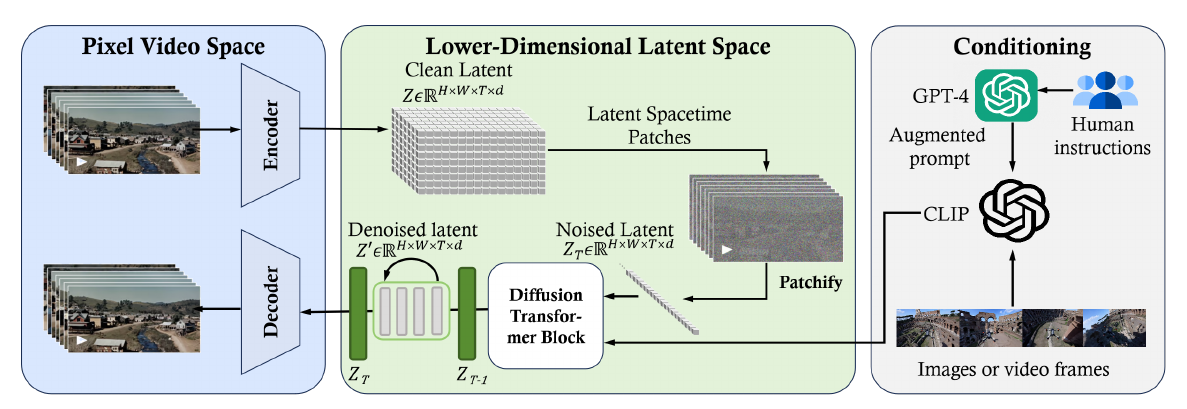
\includegraphics[width=0.9\textwidth]{images/sora_spatiotemporal_patches.png}
	\captionof{figure}{Minh họa Spatiotemporal Patches: Video được nén và chia thành các khối bao gồm thông tin không gian và thời gian, sau đó được xử lý như một chuỗi bởi Transformer.}
	\label{fig:sora_patches}
\end{center}

\textbf{Tầm ảnh hưởng:}  
Sora không chỉ là một mô hình sinh video tiên tiến; nó được xem là một bước tiến quan trọng hướng tới \textbf{Trí tuệ Nhân tạo Tổng quát (AGI)}, bởi vì nó minh họa khả năng học các mô hình thế giới từ dữ liệu video quy mô lớn, đồng thời thể hiện tiềm năng tạo ra các mô phỏng vật lý phức tạp và nhất quán. Mô hình cũng mở ra các hướng nghiên cứu mới về video generation, simulation-driven learning, và tương tác người-máy dựa trên thế giới 3D.

\subsection{Lumiere (Google, 2024): Chuyển động Mượt mà trong một Lần}
\label{subsec:lumiere}

\textbf{Lumiere} \cite{Bar-Tal2024Lumiere} từ Google Research giải quyết một trong những vấn đề cốt lõi của các mô hình Text-to-Video (T2V) trước đó: tạo ra chuyển động thực tế, mượt mà và nhất quán trên toàn bộ video.

\textbf{Triết lý và Kiến trúc:}  
Các mô hình T2V truyền thống thường tạo video bằng cách sinh một vài khung hình chính (key frames) và sau đó nội suy (interpolate) các khung hình còn lại. Phương pháp này dễ dẫn đến các chuyển động giật hoặc không tự nhiên. Lumiere thay đổi hoàn toàn cách tiếp cận này.

\begin{itemize}
	\item \textbf{Space-Time U-Net (STUNet):}
	\begin{itemize}
		\item Lumiere giới thiệu một kiến trúc U-Net không gian-thời gian, có khả năng sinh \textbf{toàn bộ video trong một lần duy nhất}.
		\item Thay vì chỉ áp dụng downsampling và upsampling theo không gian, STUNet còn bao gồm các lớp xử lý theo \textbf{chiều thời gian}, cho phép mô hình học được các mối quan hệ động lực học phức tạp.
		\item Cấu trúc này giúp mô hình nắm bắt các chuyển động dài hạn, tương tác giữa các đối tượng và giữ sự nhất quán về màu sắc, ánh sáng và hình dạng xuyên suốt video.
	\end{itemize}
	
	\item \textbf{Cơ chế hoạt động:}
	\begin{itemize}
		\item Video đầu vào được ánh xạ vào không gian tiềm ẩn (latent space) hoặc trực tiếp vào khối không gian-thời gian.
		\item STUNet thực hiện quá trình khử nhiễu diffusion trên toàn bộ khối này, sinh ra các khung hình liên tiếp đồng thời, đảm bảo tính liên tục và mượt mà của chuyển động.
		\item Nhờ việc xử lý toàn bộ khối cùng một lúc, Lumiere có khả năng duy trì các đặc trưng động nhất quán, ngay cả với các chuyển động phức tạp hoặc cảnh nhiều đối tượng.
	\end{itemize}
\end{itemize}

\textbf{Kết quả:}  
Lumiere tạo ra các video với chuyển động lớn, phức tạp và đa dạng một cách mượt mà, vượt trội hơn nhiều so với các phương pháp T2V trước đây. Nó đặc biệt hiệu quả trong các tác vụ như:
\begin{itemize}
	\item \textbf{Cinemagraphs:} Làm cho một phần của ảnh tĩnh chuyển động mà không phá vỡ tổng thể.
	\item \textbf{Stylized Generation:} Sinh video theo phong cách nghệ thuật của một ảnh hoặc video tham chiếu.
\end{itemize}

\begin{center}
	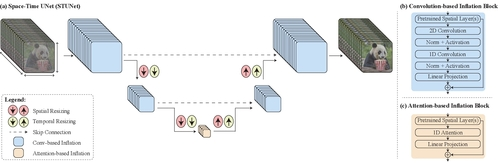
\includegraphics[width=0.9\textwidth]{images/lumiere_stunet_diagram.jpg}
	\captionof{figure}{Minh họa kiến trúc Space-Time U-Net (STUNet) của Lumiere. Mô hình xử lý toàn bộ khối không gian-thời gian của video cùng một lúc, cho phép sinh video mượt mà và nhất quán.}
	\label{fig:lumiere_stunet}
\end{center}

% Keyword gợi ý: lumiere google research, space-time unet, t2v smooth generation
\subsection{Pika Labs: Dân chủ hóa Sáng tạo Video}
\label{subsec:pika_labs}

Khác với các dự án nghiên cứu quy mô lớn như Sora và Lumiere, \textbf{Pika Labs} đại diện cho việc \textbf{sản phẩm hóa và dân chủ hóa} công nghệ Text-to-Video (T2V). Nền tảng này cho phép người dùng phổ thông tạo, chỉnh sửa và tương tác với video bằng AI một cách trực quan và nhanh chóng.

\textbf{Đặc điểm và Hướng tiếp cận:}  
Pika Labs không chỉ tập trung vào việc sinh video từ văn bản, mà còn chú trọng khả năng \textbf{tương tác và chỉnh sửa chi tiết}:

\begin{itemize}
	\item \textbf{Đa dạng đầu vào:} Người dùng có thể bắt đầu từ:
	\begin{itemize}
		\item Một prompt văn bản.
		\item Một ảnh tĩnh làm cơ sở (reference image).
		\item Một video sẵn có để chỉnh sửa hoặc tạo phiên bản mới.
	\end{itemize}
	
	\item \textbf{Khả năng chỉnh sửa tương tác:} Sau khi video được sinh, người dùng có thể tinh chỉnh từng phần cụ thể mà không cần tạo lại toàn bộ video:
	\begin{itemize}
		\item \textbf{Modify Region:} Lựa chọn một vùng cụ thể trong video và thay đổi nó theo ý muốn (ví dụ: "thay đổi màu váy thành xanh").
		\item \textbf{Expand Canvas:} Mở rộng khung hình, thêm bối cảnh xung quanh video hiện tại.
		\item \textbf{Camera Control:} Điều khiển chuyển động máy quay như pan, tilt, zoom, tạo ra cảm giác quay phim chuyên nghiệp.
	\end{itemize}
\end{itemize}

\textbf{Kiến trúc và Công nghệ nền tảng:}  
Mặc dù Pika Labs chưa công bố chi tiết kiến trúc đầy đủ, nền tảng này nhiều khả năng kết hợp:
\begin{itemize}
	\item Các mô hình diffusion hoặc transformer video tinh gọn để sinh video nhanh trên cloud.
	\item Cơ chế điều khiển tương tác (interactive control) tương tự ControlNet hoặc các điều kiện không gian-thời gian, cho phép chỉnh sửa cục bộ mà không làm ảnh hưởng toàn bộ video.
	\item Tối ưu hóa inference để có thể xử lý video độ phân giải trung bình trong thời gian thực hoặc gần thực.
\end{itemize}

\textbf{Tầm ảnh hưởng:}  
Pika Labs, cùng với các startup như Runway, đã biến T2V từ một công cụ nghiên cứu tiên tiến thành một \textbf{công cụ sáng tạo trực tiếp} cho:
\begin{itemize}
	\item Nhà làm phim và biên tập video.
	\item Nhà thiết kế nội dung số và sáng tạo trên mạng xã hội.
	\item Người dùng cá nhân muốn tạo nội dung video nhanh, tùy chỉnh và mang tính cá nhân hóa cao.
\end{itemize}
Điều này đánh dấu một bước tiến quan trọng: \textbf{T2V không còn là công nghệ thử nghiệm trong phòng thí nghiệm, mà trở thành công cụ phổ biến trong sản xuất sáng tạo hàng ngày.}

\begin{center}
	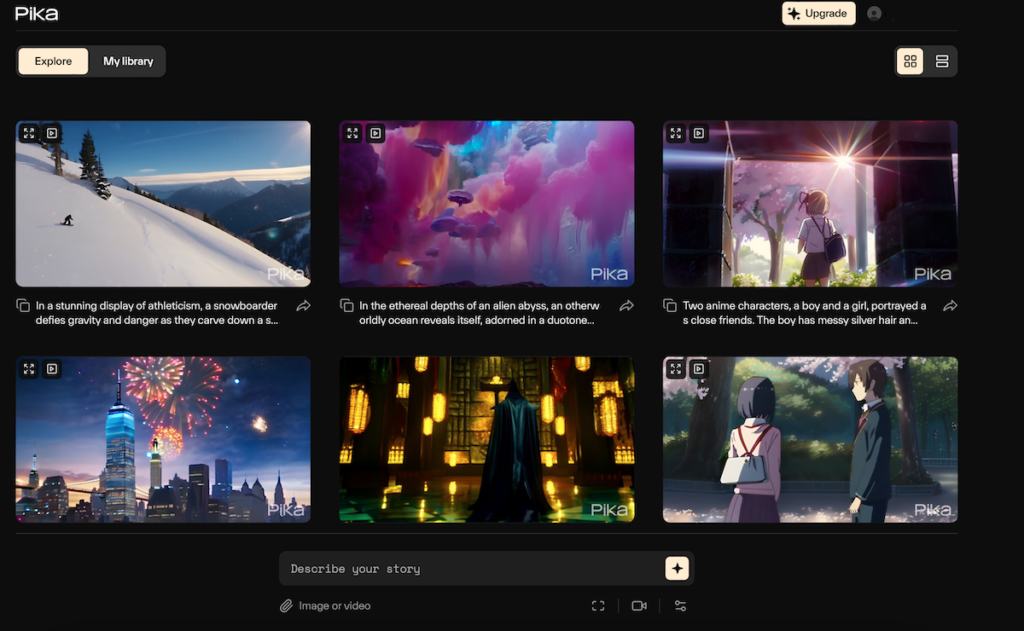
\includegraphics[width=0.9\textwidth]{images/pika_labs_interface.png}
	\captionof{figure}{Giao diện Pika Labs, minh họa các tính năng tương tác: chỉnh sửa vùng (Modify Region), mở rộng khung hình (Expand Canvas) và điều khiển máy quay (Camera Control).}
	\label{fig:pika_labs_interface}
\end{center}

% Keyword gợi ý: pika labs video ai, interactive t2v, video editing ai
\subsection{Kết luận và Tương lai}
Các mô hình Text-to-Video đã đánh dấu một bước tiến ngoạn mục trong lĩnh vực AI sáng tạo, chuyển từ việc tạo ra các hình ảnh tĩnh sang việc tổng hợp các thế giới động. Sự phát triển nhanh chóng từ các clip ngắn, giật cục đến các đoạn video dài, mượt mà và có cốt truyện như của Sora cho thấy một tương lai đầy hứa hẹn.

Xu hướng trong giai đoạn 2024-2025 đang tập trung vào:
\begin{itemize}
	\item \textbf{Video Foundation Models:} Xây dựng các mô hình T2V nền tảng, có thể được tinh chỉnh và điều khiển cho nhiều ứng dụng khác nhau.
	\item \textbf{Video dài hơn và có tính tương tác:} Hướng tới việc tạo ra các video có thời lượng dài hơn một phút, với khả năng duy trì cốt truyện và cho phép người dùng tương tác, chỉnh sửa nội dung.
	\item \textbf{Mô phỏng 3D và Điều khiển Vật lý:} Các mô hình ngày càng hiểu rõ hơn về vật lý và không gian 3D, cho phép tạo ra các video không chỉ đẹp mà còn hợp lý về mặt động học.
\end{itemize}
Các mô hình T2V không còn là công cụ tạo clip đơn thuần; chúng đang trên đường trở thành những "cỗ máy kể chuyện" (storytelling engines) và "mô phỏng thế giới" (world simulators), hứa hẹn sẽ định nghĩa lại cách chúng ta tạo ra và tương tác với nội dung số.

\section*{Tài liệu tham khảo}
\begin{itemize}
	\item[1] OpenAI. (2024). \textit{Video generation models as world simulators}. OpenAI Technical Report. (Báo cáo kỹ thuật giới thiệu Sora).
	\item[2] Bar-Tal, O., et al. (2024). \textit{Lumiere: A Space-Time Diffusion Model for Video Generation}. Google Research. (Paper giới thiệu Lumiere và kiến trúc STUNet).
	\item[3] Pika Labs. (2023). \textit{Pika 1.0 Announcement}. Pika Labs Blog \& Product Release. (Công bố sản phẩm Pika 1.0 với các tính năng tương tác).
	\item[4] Ho, J., Jain, A., \& Abbeel, P. (2020). Denoising diffusion probabilistic models. In \textit{Advances in Neural Information Processing Systems (NeurIPS)}. (Paper nền tảng về DDPM, công nghệ cốt lõi của hầu hết các mô hình T2V).
	\item[5] Rombach, R., Blattmann, A., Lorenz, D., Esser, P., \& Ommer, B. (2022). High-resolution image synthesis with latent diffusion models. In \textit{CVPR}. (Paper về Latent Diffusion, kiến trúc nền tảng được mở rộng cho video).
	\item[6] Peebles, W., \& Xie, S. (2022). Scalable diffusion models with transformers. \textit{arXiv preprint arXiv:2212.09748}. (Paper giới thiệu Diffusion Transformer - DiT, kiến trúc được cho là nền tảng của Sora).
\end{itemize}